% !TeX spellcheck = es_VE
% !TeX root = Informe.tex
% !TeX spellcheck = es_VE
\documentclass[12pt,letterpaper]{article}
\usepackage[utf8]{inputenc}
\usepackage{amsmath}
\usepackage{amsfonts}
\usepackage{amssymb}
\usepackage{graphicx}
\usepackage{url}
\usepackage{tikz}
\usepackage[shortlabels]{enumitem} % Se mantiene aquí con sus opciones
\usepackage{fancyhdr}
\usepackage[spanish]{babel}
%\usepackage[acronym]{glossaries}
%\makeglossaries

% agregar circuitos electronicos
\usepackage[siunitx, american]{circuitikz}

% comas sencillas en listing
\usepackage{textcomp}
\usepackage{upquote}
\usepackage{listings}
\lstset{upquote=true}

% dimensiones de pagina
\usepackage[left=1.5cm,top=1.5cm,right=1.5cm,bottom=2.5cm]{geometry}

% hiperenlaces
\usepackage{hyperref} % Para incluir hipervínculos
\hypersetup{urlcolor=blue,colorlinks=false,pdfborder={0 0 0}} % eliminar marco rojo en enlaces (citas, indices, pies de pagina, etc)

% permitir en la numeracion de los items agregar el numero de seccion
% (Se eliminó la línea duplicada \usepackage{enumitem} que causaba el error)
\setlist[enumerate]{label=\thesection.\arabic*. }   % numerar solo con seccion
%\setlist[enumerate]{label=\thesubsection.\arabic*. } % incluir numeracion de subsection

% otras configuraciones
\usepackage{parskip}
\setlength{\parskip}{1em} % establece el espacio entre parrafos
\setlength{\parindent}{0cm} % elimina la sangria inicial en parrafo
\usepackage{array} % ajustes adicionales para tablas
% \usepackage{pdfpages} %incluir archivos pdf en documento

% personalizacion de etiquetas
\renewcommand{\figurename}{Figura}
\renewcommand{\contentsname}{Contenido}
\renewcommand{\listfigurename}{Índice de Figuras}
\renewcommand{\listtablename}{Índice de Tablas}
\renewcommand{\lstlistlistingname}{Índice de Códigos}
\renewcommand{\tablename}{Tabla}
\renewcommand{\lstlistingname}{Código}

% pie de pagina
\renewcommand{\footrulewidth}{0.4pt}% grosor de linea del pie de pag
%\lfoot{\thepage} % texto izquierda
%\rfoot{\thepage} % texto derecha
\cfoot{\thepage} % texto al centro

%% definiciones para insertar codigo de programacion al doc
\usepackage{color}
\definecolor{dkgreen}{rgb}{0,0.6,0}
\definecolor{gray}{rgb}{0.5,0.5,0.5}
\definecolor{mauve}{rgb}{0.58,0,0.82}
\lstset{frame=tb,
    language=Python,
    aboveskip=3mm,
    belowskip=3mm,
    showstringspaces=false,
    columns=flexible,
    basicstyle={\small\ttfamily},
    %numbers=left,
    numberstyle=\tiny\color{gray},
    keywordstyle=\color{blue},
    commentstyle=\color{dkgreen},
    stringstyle=\color{mauve},
    breaklines=true,
    breakatwhitespace=true,
    tabsize=3
} % fin de codigo de programacion

%%%%%%%%%%%%%% MACRO PARA CONTROL DE PUNTAJE %%%%%%%%%%%%%%%%%%
\usepackage{xifthen}
\newcounter{puntos}
\setcounter{puntos}{0} % Inicializa el contador a cero

\newcommand{\sumarPunto}[1]{%
    \addtocounter{puntos}{#1}%
    \ifthenelse{#1 > 1}{(\textbf{#1 puntos})}{(\textbf{#1 punto})} 
}
%%%%%%%%%%%%%%%%%%%%%%%%%%%%%%%%%%%%%%%%%%%%%%%%%%%%%%%%%%

%%%%%%%%%%%%%%%%%%%%%%%%%%%%%%%%%%%%%%%%%%%%%%%%%%%%%%%%%%%%%%%%%%%%%%%
\pagestyle{fancy}
\fancyhf{}

\setlength{\headheight}{80pt}
\addtolength{\topmargin}{-35pt}
\setlength{\headsep}{1cm}
\setlength{\footskip}{20pt}

\rhead{
\includegraphics[width=1.3cm]{../img/logo_ciencias.png}}
\lhead{
\includegraphics[width=1.4cm]{../img/logo_ucv.png}}
\cfoot{\thepage}
\rfoot{Junio, 2026}

\chead{Laboratorio de Internet de las Cosas}
\newcommand{\titulo}{LABORATORIO 2}
\newcommand{\subtitulo}{Comunicación Serial y Pines Analógicos en ATmega2560}
\newcommand{\autorUno}{Luisdavid Colina V24766381}
\newcommand{\autorDos}{Samantha Ramírez V31307714}
%%%%%%%%%%%%%%%%%%%%%%%%%%%%%%%%%%%%%%%%%%%%%%%%%%%%%%%%%%%%%%%%%%%%%%%
\begin{document}

%%%%%%%%%%%%%%%%%%%%%%%%%%%%%%%%%%%%%%%%%%%%%%%%%%%%%%%%%%%%%%%%%%%%%%%
\begin{center}
  {\Large \textbf{\titulo}} \\[0.3cm]
  {\large \textbf{\subtitulo}} \\[0.8cm]
  
  \small
  \begin{tabular}{c}
    \textbf{Preparado por:} \\
    \autorUno \\
    \autorDos \\
  \end{tabular}
  \\[1cm]
\end{center}

%%%%%%%%%%%%%%%%%%%%%%%%%%%%%%%%%%%%%%%%%%%%%%%%%%%%%%%%%%%%%%%%%%%%%%%
\section{Desarrollo de actividades}

\subsection{Actividad 4.7 y 4.8: Control de iluminación usando ADC y PWM}
\textit{Enunciado: Utilizando una fotoresistencia, modifique la intensidad de un led conectado a un pin digital apropiado que permita la simulación de una salida analógica, recuerda colocar la resistencia de protección entre el pin y el led. La intensidad será modificada en función de la intensidad capturada por el fotoresistor que será conectado a una entrada analógica. Al iniciar la placa el led debe estar apagado y se procederá a aumentar la intensidad del led según varíen los valores en el pin analógico. Modifique el código anterior, utilizando la instrucción map(), para que la salida del led sea ajustada a los valores máximos y mínimos obtenidos por la foto-resistencia (note que esto dependerá de la iluminación del espacio). A manera referencial puede apoyarse del Código 1 que se muestra en la sección de “Anexos”.}

En el diseño del circuito (Figura~\ref{fig:evidencia1}) se conectaron 5V a un extremo de la fotorresistencia y el otro extremo al pin A0 (entrada analógica) en serie con una resistencia a GND. Esto se hizo para que el ADC del microcontrolador pudiera traducir los cambios de resistencia física del sensor en variaciones de voltaje procesables.
Por su parte, el LED se conectó al pin digital 6 porque posee hardware dedicado para PWM, una técnica que enciende y apaga el pin digital tan rápido que simula un voltaje variable. Al ajustar qué tanto tiempo permanece encendido el pin (ciclo de trabajo), el sistema regula la energía enviada al LED de forma suave. Esto permite que el brillo cambie de manera fluida y proporcional a la luz que detecta el sensor.

\begin{figure}[ht!]
    \centering
    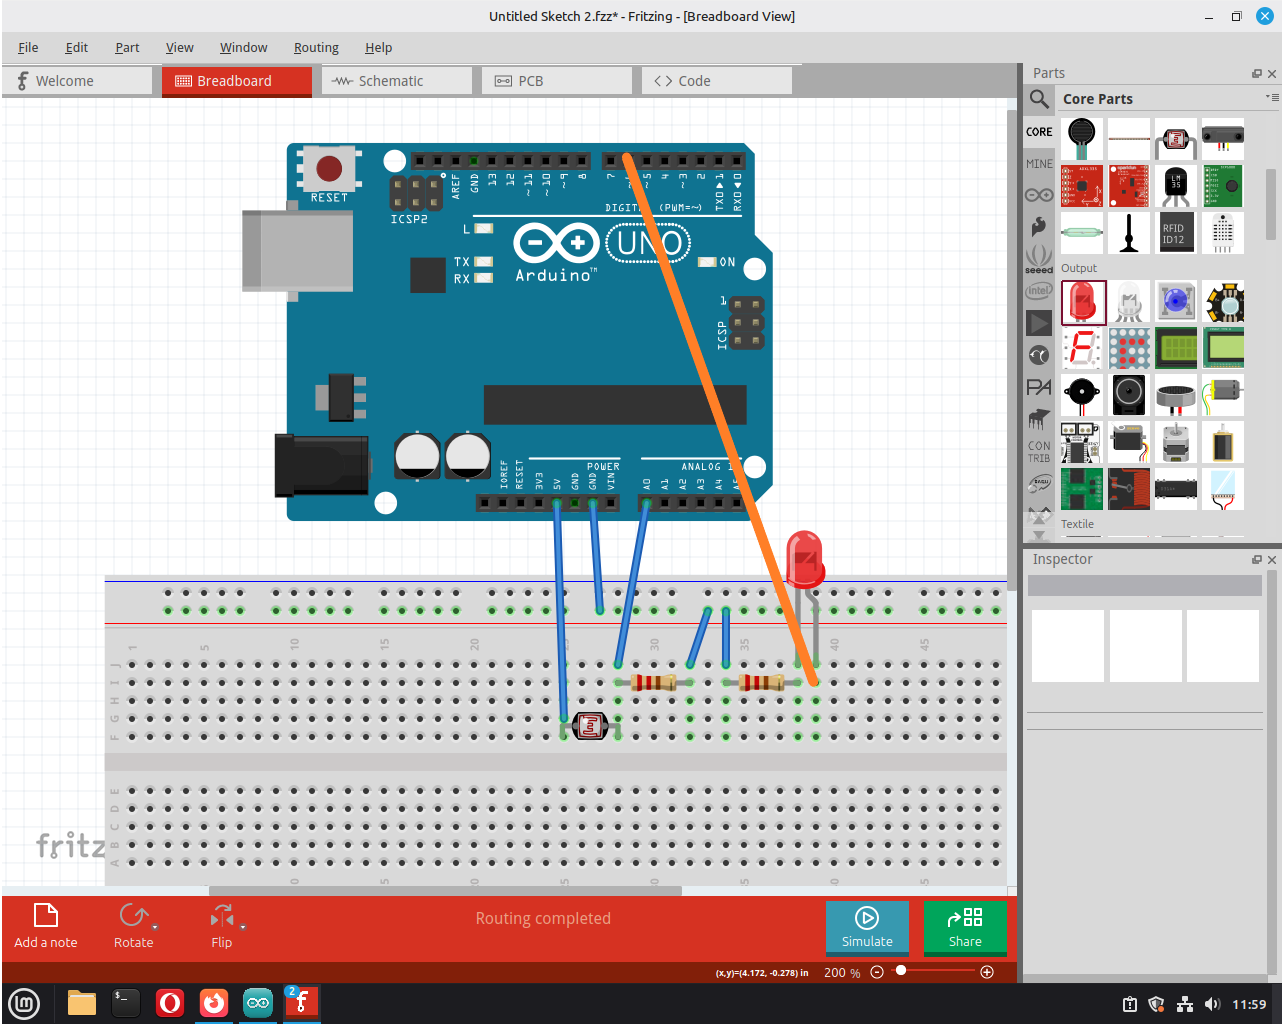
\includegraphics[width=0.8\linewidth]{img/evidencia1.png}
    \caption{Diseño del circuito en Fritzing.}
    \label{fig:evidencia1}
\end{figure}
\begin{figure}[ht!]
    \centering
    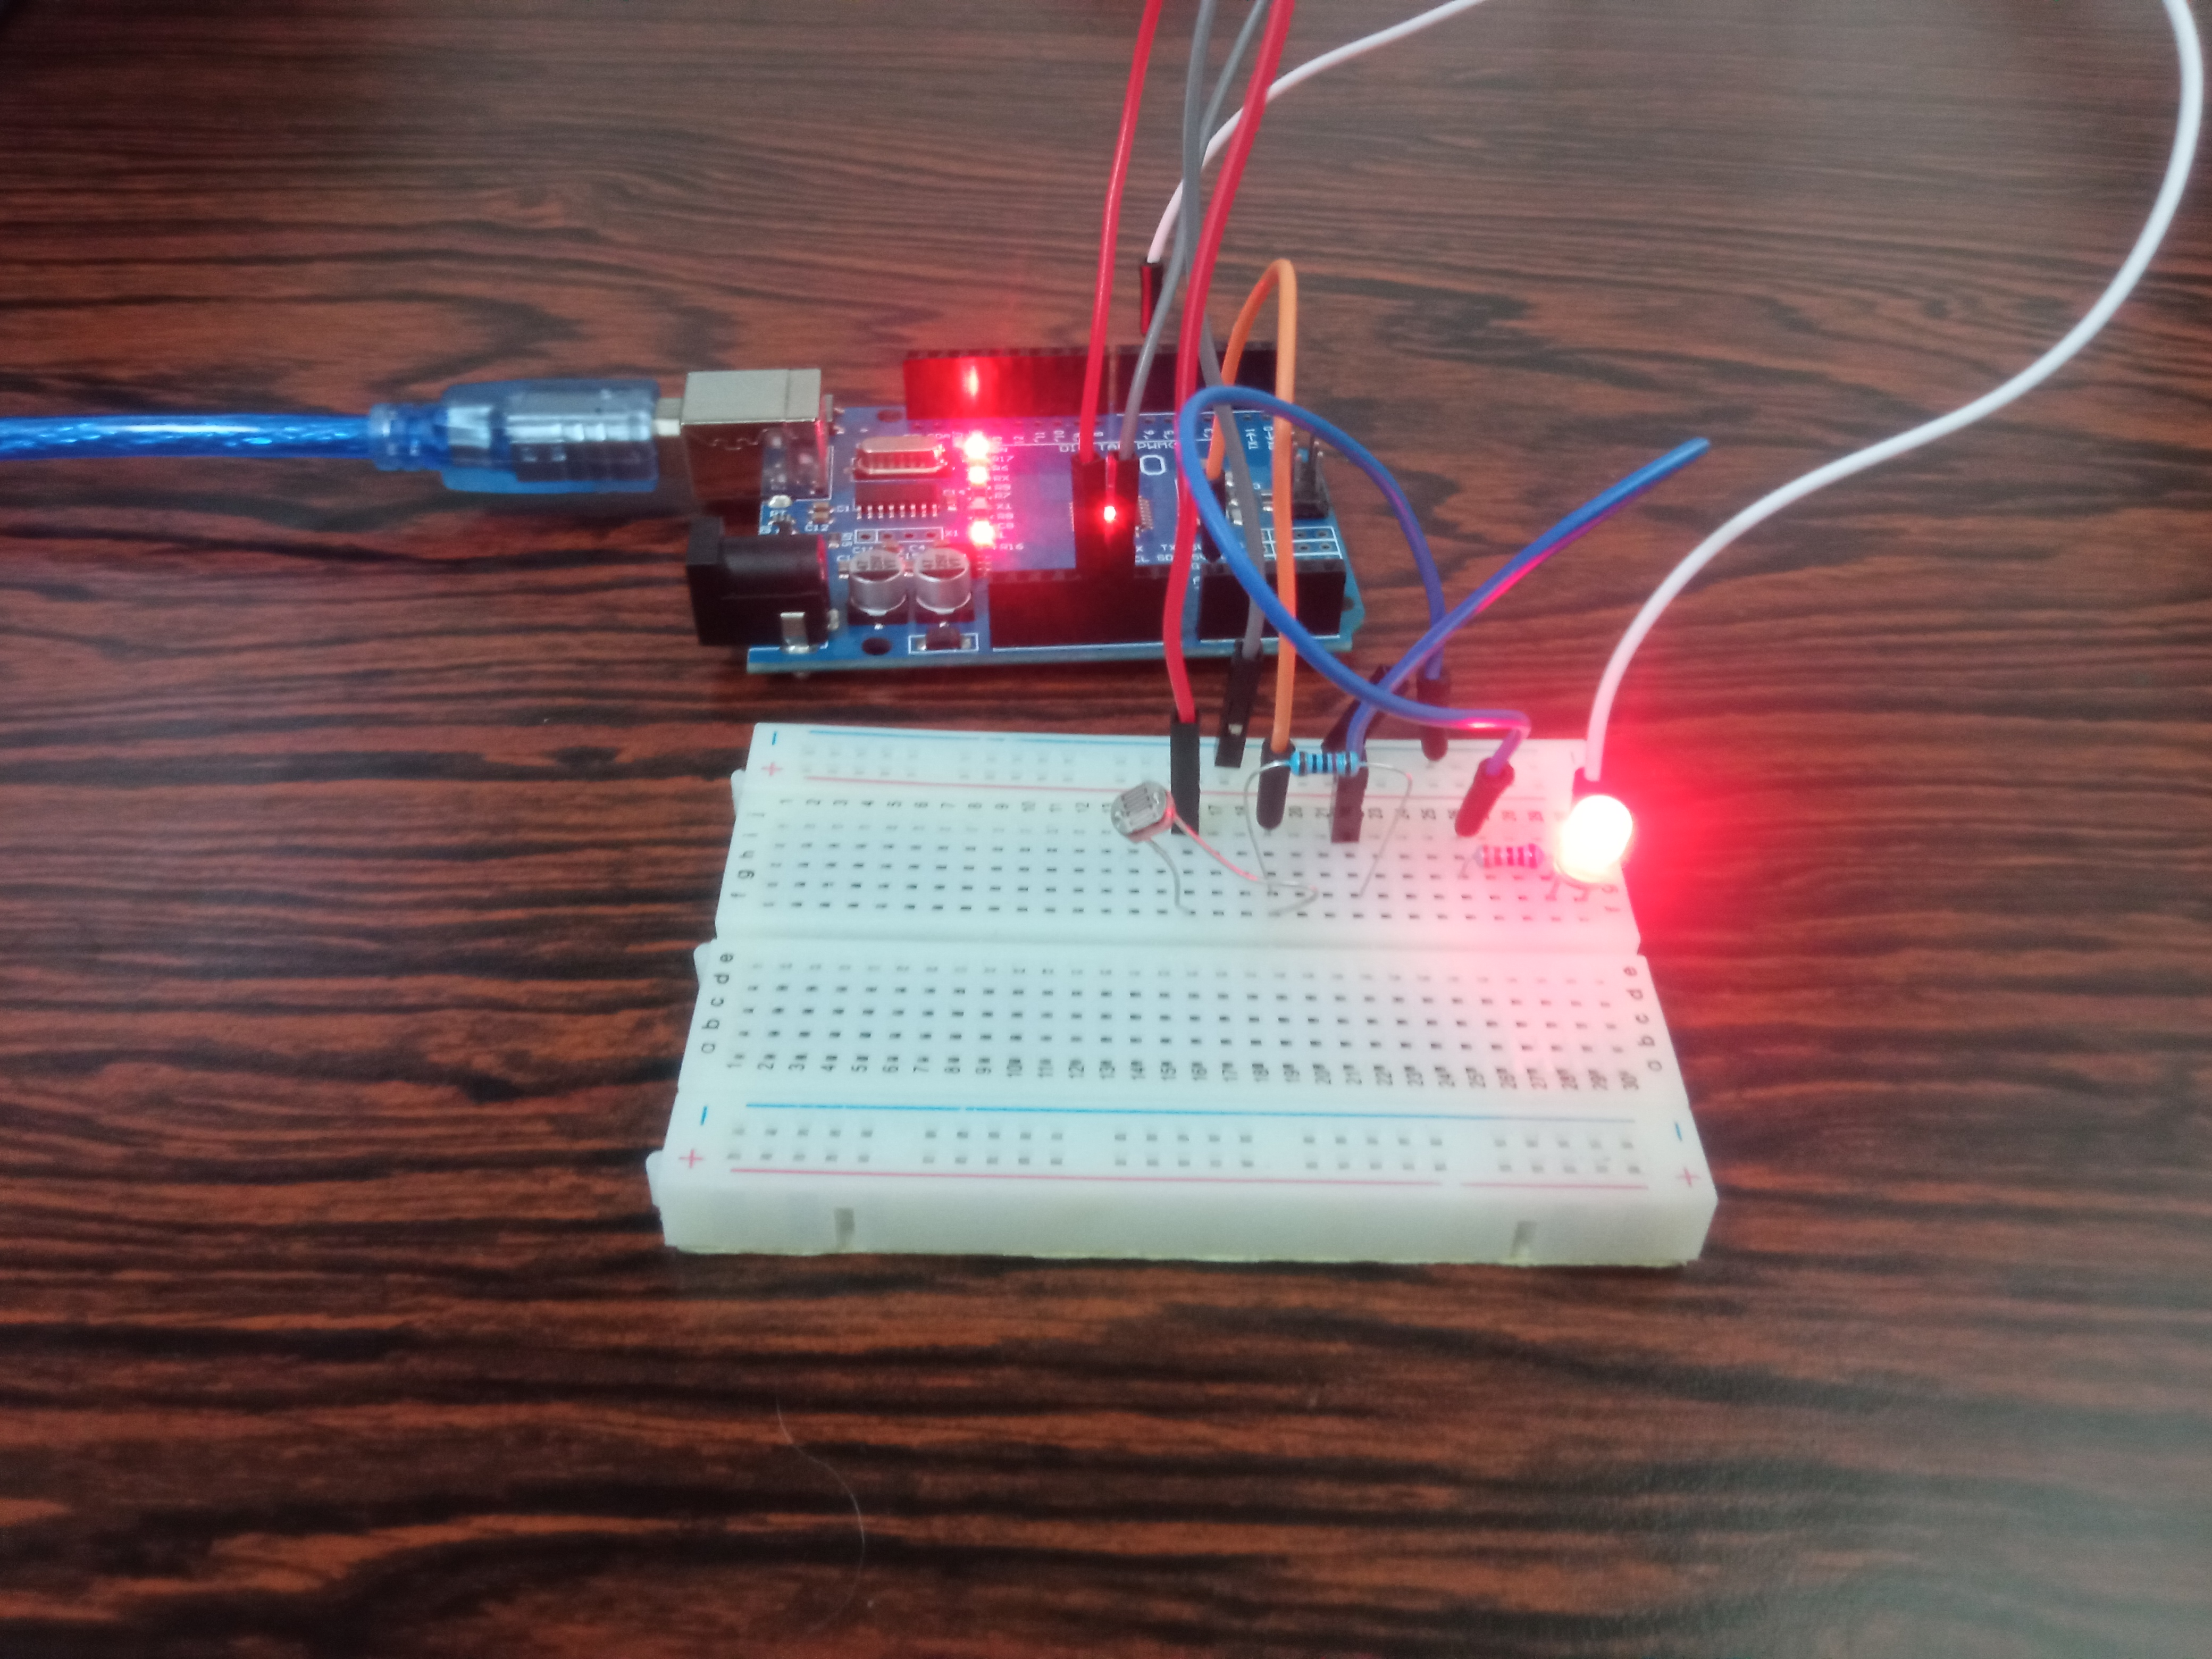
\includegraphics[width=0.6\linewidth]{img/evidencia3.jpg}
    \caption{Circuito armado en físico.}
    \label{fig:evidencia3}
\end{figure}

\pagebreak
La implementación real (Figura~\ref{fig:evidencia3}) se rige por el código fuente (Figura~\ref{fig:evidencia2}), el cual establece el flujo de datos desde la captura hasta la actuación. Inicia con la vinculación del \texttt{lldrPin} al puerto analógico A0 y el \texttt{lledPin} al puerto digital 6. Dentro del ciclo principal, la instrucción \texttt{analogRead(ldrPin)} activa el ADC de 10 bits para cuantificar la tensión del sensor, almacenando el valor digitalizado en \texttt{lvalorLDR}. Se utiliza la función \texttt{map()}, que escala linealmente el rango dinámico detectado en el laboratorio (145-800) a la resolución de 8 bits (0-255) requerida por el hardware de salida del microcontrolador.

El ADC ayuda traducir voltaje en datos binarios discretos que la CPU de 8 bits pueda procesar. El rango de valores obtenido en el pin analógico es de 0 a 1023 por su resolución de 10 bits ($2^{10}$ combinaciones), mientras que la escritura en el pin digital PWM está limitada a un rango de 0 a 255.

\begin{figure}[ht!]
    \centering
    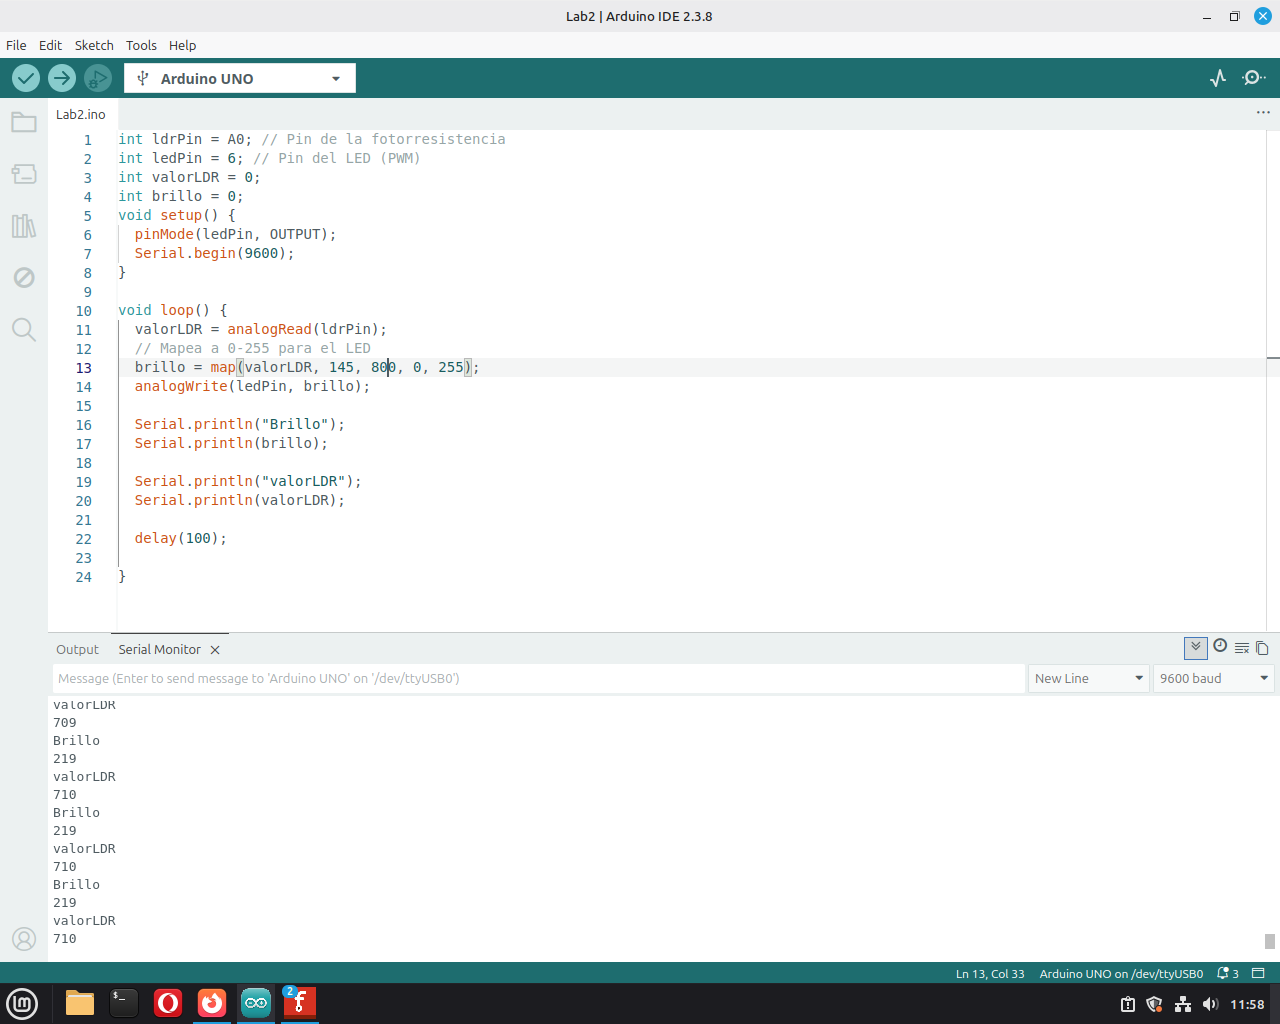
\includegraphics[width=0.8\linewidth]{img/evidencia2.png}
    \caption{Código fuente en el IDE de Arduino.}
    \label{fig:evidencia2}
\end{figure}

\pagebreak
Las Figuras~\ref{fig:evidencia4}, \ref{fig:evidencia5}, \ref{fig:evidencia6}, \ref{fig:evidencia7} confirman que el sistema funciona correctamente: al tapar el sensor con un dedo, la intensidad del LED disminuye de forma inmediata. Técnicamente, esto sucede porque al haber menos luz, la resistencia del sensor aumenta y el voltaje en el pin A0 baja; el programa detecta esta caída y reduce la potencia enviada al LED.

Los datos del Monitor Serial validan esta precisión, mostrando cómo una lectura de 710 en el sensor se convierte fluidamente en un brillo de 219. Gracias a la comunicación en tiempo real, se comprobó que el brillo del LED se ajusta de manera suave y proporcional a los cambios de luz en el laboratorio.

\begin{figure}[ht!]
    \centering
    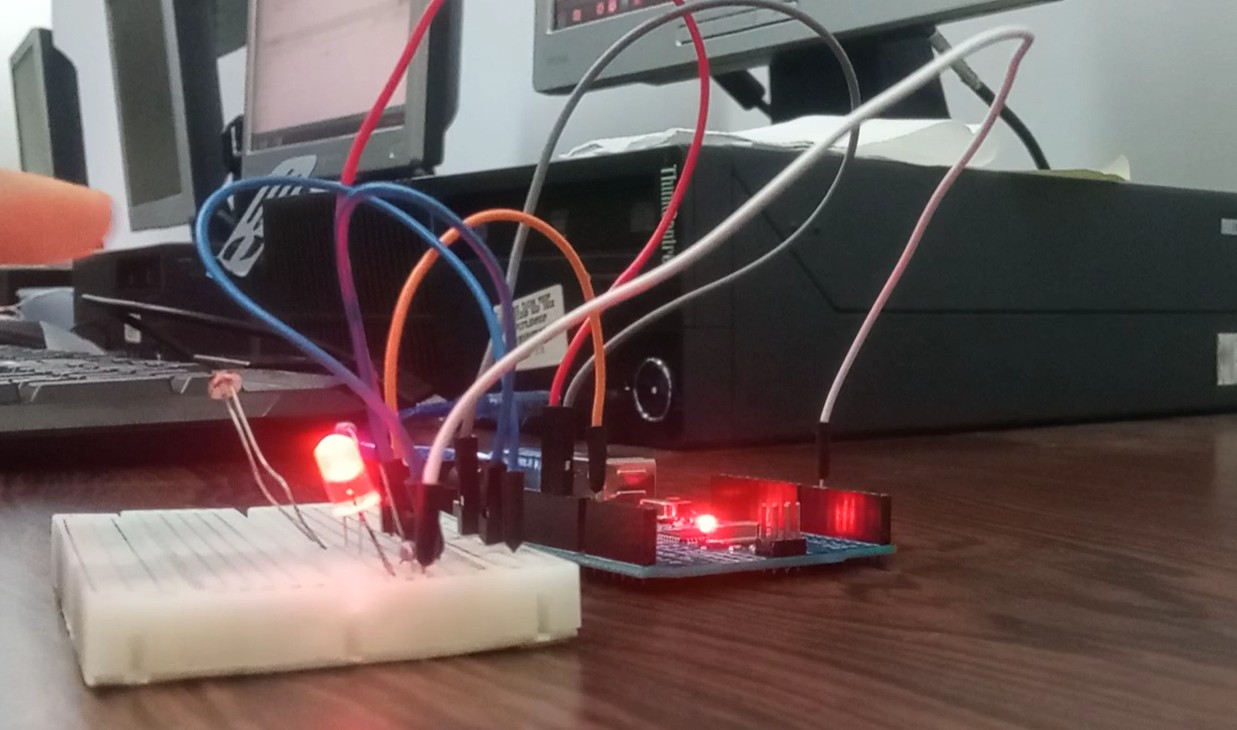
\includegraphics[width=0.5\linewidth]{img/evidencia4.jpg}
    \caption{Led con alta intensidad al fotoresistor recibir más luz.}
    \label{fig:evidencia4}
\end{figure}
\begin{figure}[ht!]
    \centering
    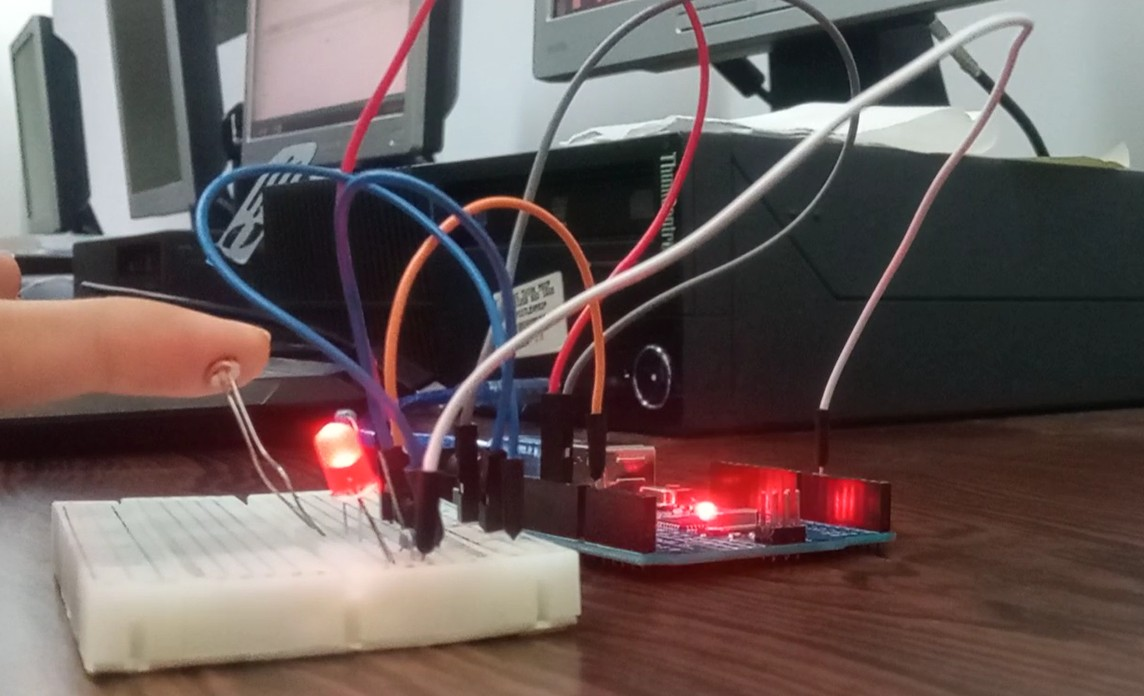
\includegraphics[width=0.5\linewidth]{img/evidencia5.jpg}
    \caption{Led con baja intensidad al fotoresistor recibir menos luz.}
    \label{fig:evidencia5}
\end{figure}
\begin{figure}[ht!]
    \centering
    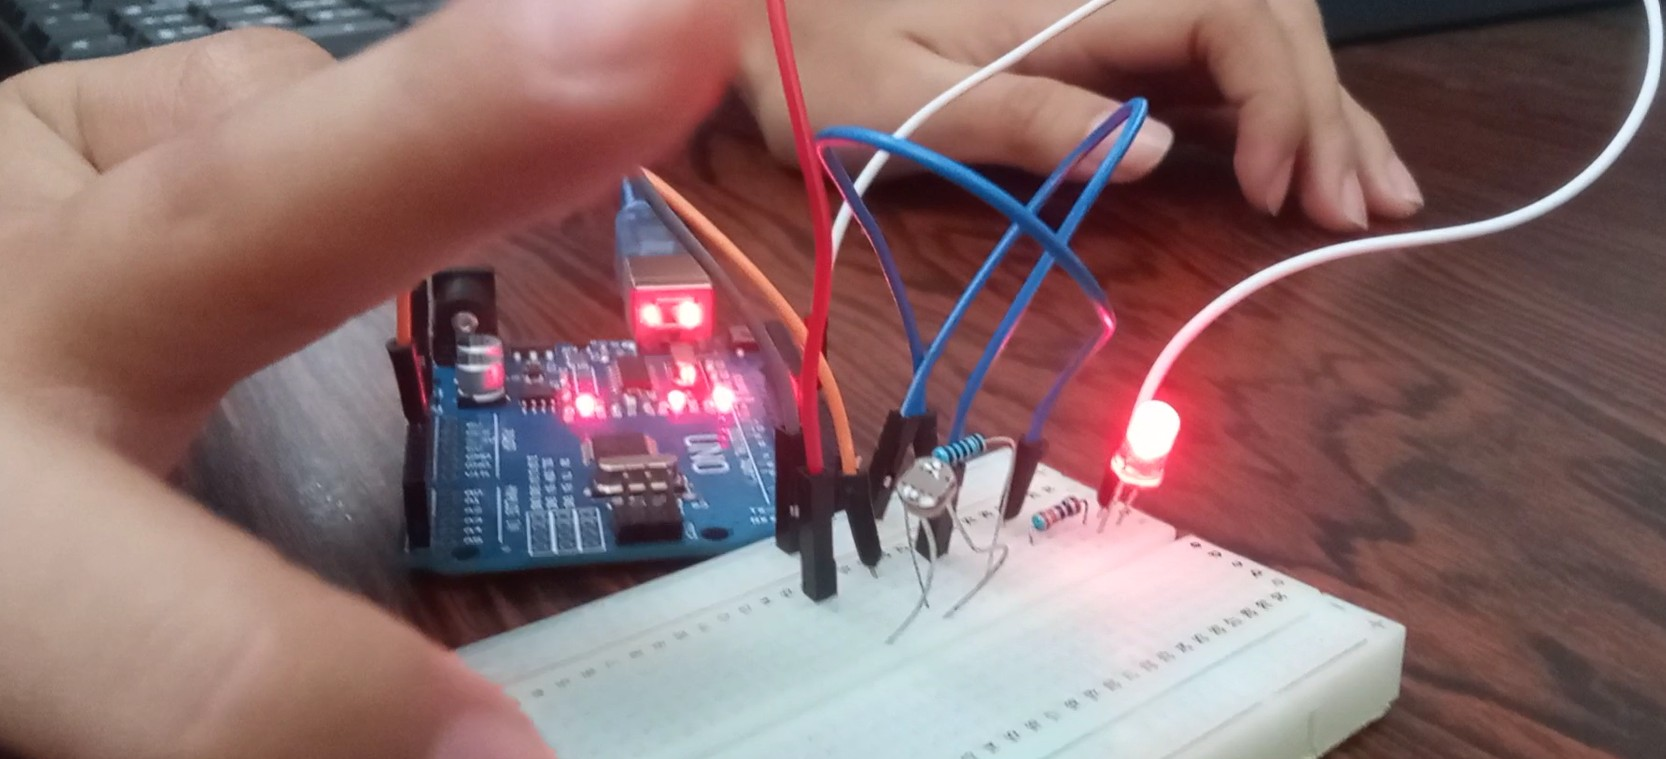
\includegraphics[width=0.5\linewidth]{img/evidencia6.jpg}
    \caption{Led con alta intensidad al fotoresistor recibir más luz.}
    \label{fig:evidencia6}
\end{figure}\begin{figure}[ht!]
    \centering
    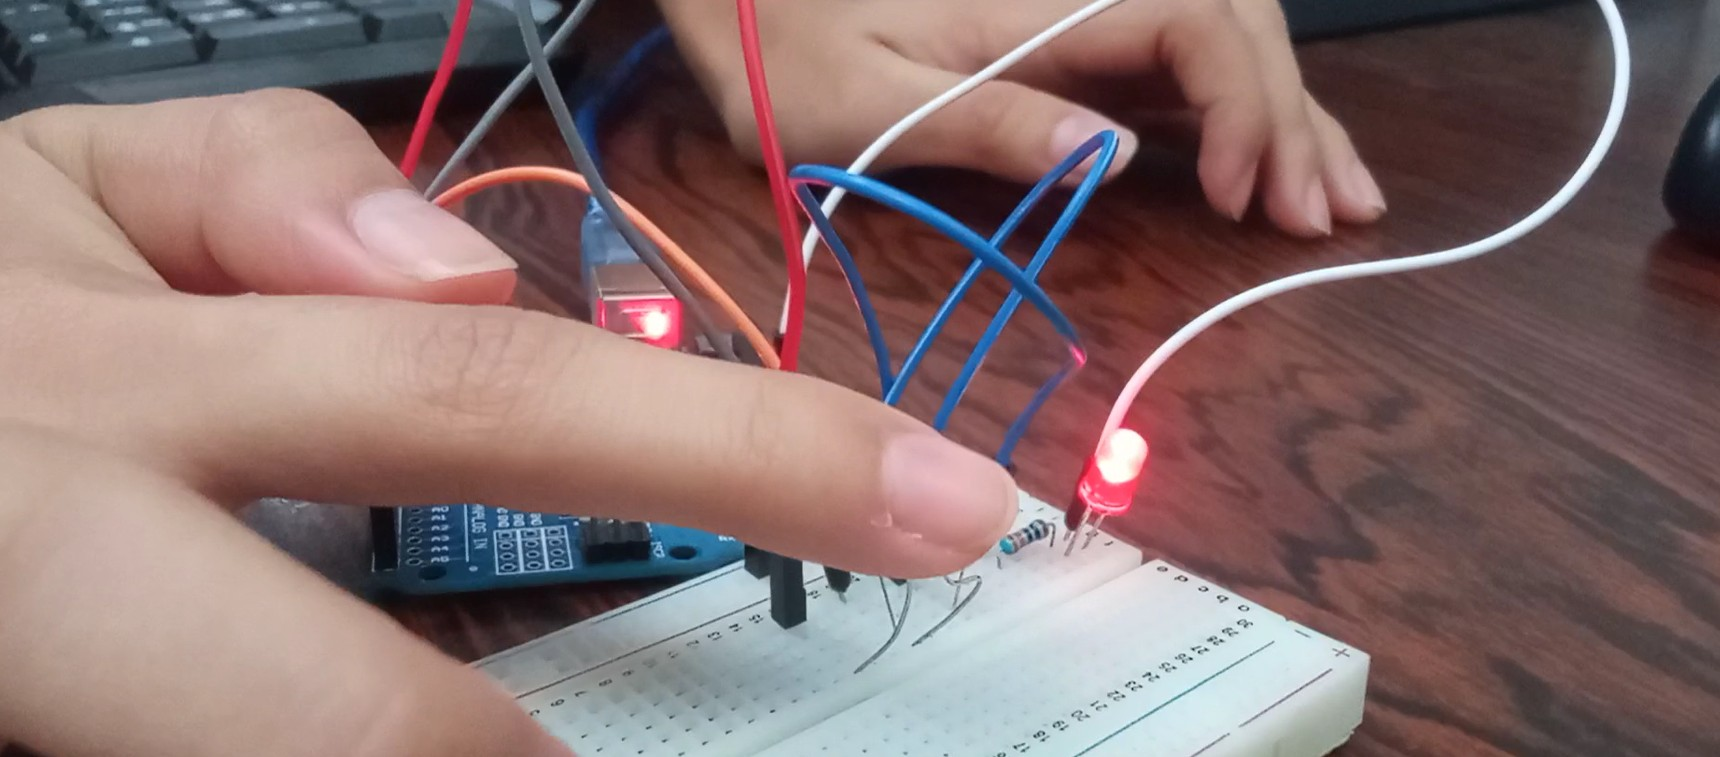
\includegraphics[width=0.5\linewidth]{img/evidencia7.jpg}
    \caption{Led con baja intensidad al fotoresistor recibir menos luz.}
    \label{fig:evidencia7}
\end{figure}

%%%%%%%%%%%%%%%%%%%%%%%%%%%%%%%%%%%%%%%%%%%%%%%%%%%%%%%%%%%%%%%%%%%%%%%
\section{Conclusiones}
Para concluir, la práctica demuestra que la arquitectura del ATmega2560 permite una integración eficiente entre el entorno físico y el digital mediante el procesamiento de señales mixtas. Se validó que el ADC de 10 bits es el componente esencial para traducir magnitudes analógicas continuas, como la luz captada por la fotorresistencia, en datos digitales procesables (rango 0-1023).

Asimismo, el uso de la técnica PWM en los pines digitales permite emular voltajes variables para controlar actuadores de forma fluida, regulando la potencia del LED según las condiciones del entorno. Finalmente, se determinó que la función map() es una herramienta técnica crítica para normalizar los datos y garantizar la interoperabilidad entre periféricos de distinta resolución, alineando la entrada del sensor con la capacidad de salida de 8 bits del hardware.

%%%%%%%%%%%%%%%%%%%%%%%%%%%%%%%%%%%%%%%%%%%%%%%%%%%%%%%%%%%%%%%%%%%%%%%
\begingroup
\small
\begin{thebibliography}{9}

\bibitem{unoboard}
Arduino, ``Arduino UNO Rev3 --- Datasheet and Schematics,''
\emph{Arduino Hardware Documentation}, Arduino LLC, Ivrea, Italia, 2023.
[En línea]. Disponible: \url{https://docs.arduino.cc/hardware/uno-rev3}.
[Consulta: jun.~2026]

\end{thebibliography}
\endgroup

\end{document}